\chapter{Rationale}\label{chap:rationale}

\section{Introduction}

The research project, titled ``\makeatletter\@title\makeatother,'' is a child project within the broader MOOD-Sense initiative. The MOOD-Sense project employs \gls{IoT} devices to detect and predict challenging behavior in dementia patients. The project aims to develop an early warning system combining sensors, artificial intelligence, and wireless communication to provide feedback for healthcare professionals and improve patient care and safety \cite{MOOD-Sense_Research}. To further enhance the connectivity and scalability among \gls{IoT} devices in the MOOD-Sense project, a new network protocol called Thread is proposed to be implemented. Thread is a low-power, IPv6-based, mesh networking protocol specifically designed for \gls{IoT} applications, offering secure, reliable, and efficient communication. It supports self-healing networks with robust routing capabilities and features like end-to-end encryption, making it an ideal choice for the MOOD-Sense initiative \cite{Thread_Group_Benefits}.

The primary focus of this child project is to optimize the energy efficiency of the wireless Thread network protocol utilized by various wireless sensors and MOOD-Sense projects. To achieve this goal, the project examines transmission power network parameters and configuration aspects, such as device types, path loss, positions, and \gls{RSSI}. Thread supports multiple device types, including border routers, leader, routers, and end devices, each serving distinct roles in the network. Border routers enable communication between the Thread network and external networks, the leader is responsible for managing network-wide configurations, routers facilitate data routing within the network, and end devices are typically low-power devices that transmit and receive data \cite{Thread_Group_Fundamentals}. By optimizing the configuration of these devices, the project aims to enhance energy efficiency. Through the establishment of a Thread network and the employment of an algorithmic approach using appropriate hardware, this research investigates the impact of transmission power network parameter optimization on maintaining reliable communication between devices while minimizing power consumption. Ultimately, the project aims to develop more energy-efficient \gls{IoT} networks to improve the performance of the MOOD-Sense initiative.


\section{Present Situation}\label{sec:present_situation}
The MOOD-Sense research project originally planned to use three wireless communication technologies: \gls{BLE}, ZigBee, and Wi-Fi for network communication. However, without a central network protocol, various subprojects within MOOD-Sense, such as dementia patient behavior registration and environmental context monitoring, are being carried out separately. This separation leads to disconnected devices and makes data sharing and integration difficult. The current situation in the lab setup can be visualized as a diagram showing isolated subprojects and devices without an integrated network.

\begin{figure}[H]
    \centering
    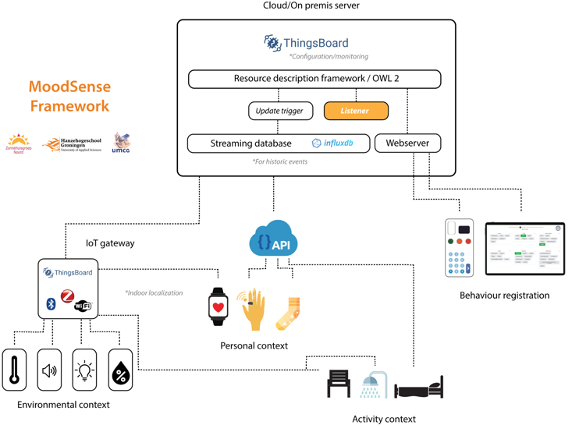
\includegraphics[width=0.8\textwidth]{images/rationale/rationale_present_situation.png}
    \caption{Current state of the MOOD-Sense initiative.}
    \label{fig:rationale_present_situation}
\end{figure}

To address these challenges and create an energy-efficient network, the proposal to implement a Thread mesh wireless network was introduced. Thread's features, such as mesh networking, multiprotocol support, and low cost, make it an ideal solution for connecting \gls{BLE}, ZigBee, and Wi-Fi connectivity together \cite{Semiconductor_Nordic_Product_Brief_2018_2.0}. However, Thread devices can consume more power than other network types due to frequent activity needed for processing data from sensors or other end devices \cite{semiconductor_battery_2021}. For instance, a sensor constantly monitoring a dementia patient's activity and sending data through the network at a very high frequency. This situation could lead to higher electricity costs and shorter device lifespans.

Optimizing the overall power consumption in the Thread network can save on electricity bills, extend device lifetimes, and enable the use of portable batteries to power the network when grid electricity isn't available. In settings like nursing homes where MOOD-Sense applications are deployed, reducing overall \gls{IoT} network power consumption can significantly cut down electricity costs, making the system more cost-effective for care facilities. Additionally, this research aligns with sustainable research principles, reducing environmental impact by cutting down energy use. The research aims to create an energy-efficient and reliable Thread mesh wireless network for \gls{IoT} applications like MOOD-Sense.


\section{Desired Outcome}\label{sec:desired_outcome}
The desired outcome of this research is to develop an efficient algorithm that integrates seamlessly within the Thread-based wireless network system and optimizing power consumption. This algorithm will not only adjust transmission power but also select the most suitable device types for the network, contributing to energy efficiency and reliable communication. A schematic overview of the system with the integrated algorithm is as follows:

\begin{figure}[H]
    \centering
    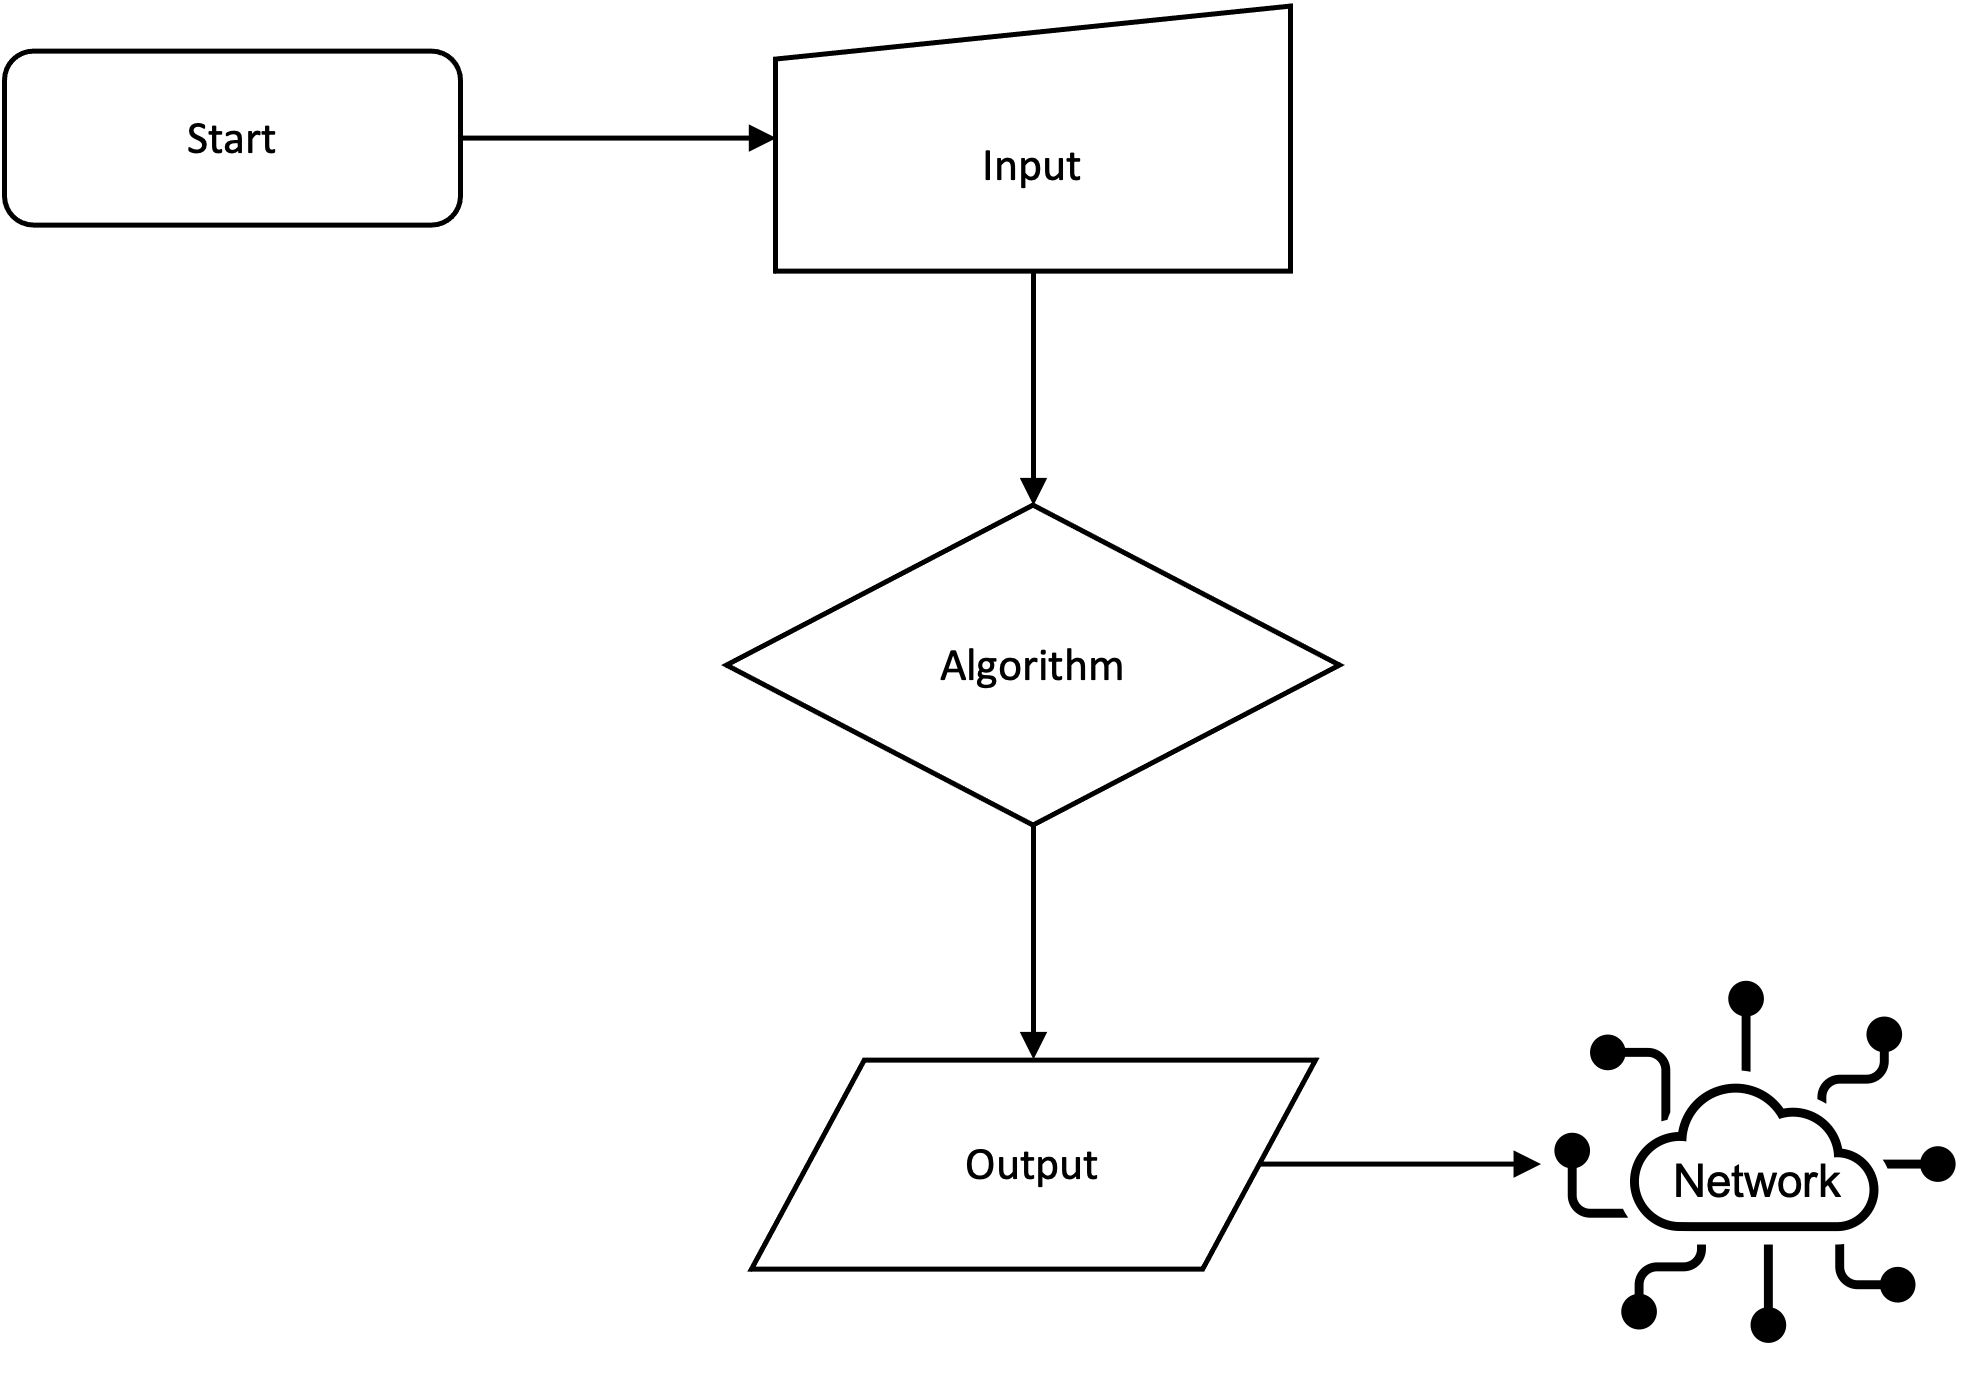
\includegraphics[width=0.8\textwidth]{images/rationale/desired-outcomes.png}
    \caption{Schematic overview of desired outcomes.}
    \label{fig:rationale_desired_outcomes}
\end{figure}

\begin{enumerate}
    \item \textbf{Input}: The primary input parameters for the network optimization algorithm include the total number of devices, the distance between each device, and network parameters. These inputs provide the necessary data to guide the optimization process and ensure that the algorithm makes informed decisions regarding device types and transmission power levels.
    \item \textbf{Algorithm}: The power optimization algorithm consists of two stages: the \acrfull{MCM} and the \acrfull{GA}. \gls{MCM} and \gls{GA} were chosen due to their ability to efficiently solve complex optimization problems that involve multiple variables and constraints. \gls{MCM} is particularly effective in dealing with uncertainty and randomness in optimization problems, while \gls{GA} offers a robust solution for finding optimal values in large search spaces \cite{kroese2014monte}. In the first stage, \gls{MCM} focuses on determining the right device types based on various constraints and constructing an optimal network configuration with an initial transmission power setting. The second stage involves \gls{GA}, which takes the output from \gls{MCM} and optimizes the transmission power settings to minimize power consumption while maintaining network reliability. One of \gls{GA}'s key strengths is its ability to avoid local optima and explore the search space more thoroughly, increasing the likelihood of finding global optima for the problem at hand \cite{lambora2019genetic}.
    \item \textbf{Output}: The output consists of the appropriate device types for a reliable Thread network configuration, along with the optimal transmission power settings for each device, and device positions. This output enables the creation of an energy-efficient and reliable Thread-based wireless network that meets the needs of the MOOD-Sense initiative and other similar \gls{IoT} applications.
    \item \textbf{Integration}: The output from the algorithm for optimal devices and roles within the network, such as border routers, routers, and end devices, will be integrated into the Thread network through a manual configuration process. Additionally, the optimal transmission power settings, as determined by the algorithm, will be applied to each device to minimize power consumption while maintaining network reliability. This manual configuration process ensures that the devices are set up for optimal performance based on the algorithm's recommendations. In the future, automated integration could be explored to streamline this process further.
\end{enumerate}

By achieving this desired outcome, the algorithm will provide a comprehensive solution for power optimization in Thread networks, supporting the MOOD-Sense initiative and similar IoT applications in building energy-efficient and sustainable networks.


\section{Problem Definition}\label{sec:problem_definition}
As the adoption of \gls{IoT} devices in applications like the MOOD-Sense initiative increases, there is a growing need for energy-efficient and reliable wireless network protocols. The Thread network protocol offers low-power and reliable mesh networking, making it suitable for such applications \cite{Thread_Group_Fundamentals}. However, optimizing power consumption while maintaining network reliability remains a challenge. Additionally, the selection of appropriate device types is crucial for building an efficient Thread network, as Thread offers various device types depending on the use case.

The primary goal of this research is to determine the most effective algorithmic approach for power optimization in a Thread-based wireless network, specifically through transmission power adjustments and the selection of the appropriate device types. By focusing on these aspects, the research will contribute to the development of energy-efficient network solutions for the MOOD-Sense initiative and similar \gls{IoT} applications. This approach ensures the proper selection and utilization of devices within the Thread network, optimizing the overall network performance and energy efficiency.


\section{Main Research Question}
How can parameter optimization be applied to develop a power-optimized Thread mesh wireless network?


\section{List of Requirements}\label{sec:list_of_requirements}
\begin{enumerate}
    \item Optimize power efficiency for the Thread network protocol with a focus on minimizing power consumption while maintaining reliable communication, and assess the impact of location on power optimization performance for both maximum and optimized modes.\\
    \textbf{Constraint}: The optimization should not compromise the network's stability, communication quality, or applicability to diverse environments.
    \item Employ \gls{MCM} and \gls{GA} for optimizing transmission power, determining efficient network configurations, investigating the significance of errors in the power optimization process, and evaluating their impact on the performance of \gls{MCM} and \gls{GA} modes.\\
    \textbf{Constraint}: The optimization techniques should be computationally feasible, not add significant overhead to the network's operation, and should identify potential sources of errors while recommending ways to minimize their impact on power optimization performance.
    \item Develop a power-optimized Thread mesh wireless network by considering the optimal device types for different nodes, and compare the performance of \gls{MCM} and \gls{GA} modes across different device types and locations in terms of power optimization.\\
    \textbf{Constraint}: The selected device types should maintain low power consumption while meeting the network's performance requirements, and the comparison should be fair and unbiased.
    \item Suggest future research directions and improvements for Thread network optimization, including device positioning, path loss, and broader application scope, while ensuring adherence to responsible research and innovation principles, including ethical aspects, professional skills, applied research, and sustainability.\\
    \textbf{Constraint}: The suggestions should be realistic and feasible, considering existing limitations and challenges in the field, and the research should prioritize the development of sustainable solutions and maintain transparency and accountability throughout the process.
\end{enumerate}


\section{Sub-Research Questions}
\begin{enumerate}
    \item What are the key features of the Thread protocol that make it suitable for \gls{IoT} applications, specifically in the context of the MOOD-Sense project, and what are the specific hardware requirements for implementing a Thread network?
    \item Which parameters significantly impact the transmission power in a Thread network, and how do they relate to energy efficiency and network performance?
    \item How do the \gls{MCM} and the \gls{GA} differ in their approach to optimizing transmission power in a Thread network, and what are the key steps for their implementation? How do variations in algorithmic parameters impact their performance?
    \item What are the differences in power optimization performance between different iterations for both maximum and optimized modes, and how do various factors such as device performance, location, device types, and the correlation between mean, max, and min Current $\left(mA\right)$ values impact the optimization process?
    \item How do \gls{MCM} and \gls{GA} modes compare with maximum mode in terms of efficiency across various locations and device types, and what is the significance of errors in the power optimization process and their impact on the performance of \gls{MCM} and \gls{GA} modes?
\end{enumerate}
